\chapter{Implementace webové aplikace}
\label{chap:implementation}

Vytvořený nástroj je editor ve formě webové aplikace. Ke zformování byly použité výše popsané technologie Angular a Konva.js. 
Jedná se o tzv. \emph{single page application (SPA)}, kde veškerý obsah a funkcionalita se nachází pouze na straně klienta a neexistuje žádný
serverový backend. Řízení stavů je vyřešeno pomocí sdílené služby, která uchovává potřebná data k vykreslování objektů na plátno.
Stavy jsou při každém potřebném překreslení aktualizovány. Díky tomuto lze celý projekt jednoduše uložit do souboru a kdykoli znovu načíst.
    
\section{Vykreslování plátna}
    O vykreslování se stará několik služeb frameworku Angular dohromady. Důvod je ten, že k určitým objektům je nutno změnit způsob jakým jsou vytvořeny a vykresleny.
    Informace o tom, co se má vykreslit, jsou jim předávány přes komponenty, které mají služby v sobě injektované. Tyto komponenty reagují
    na změny v rozhraní provedené uživatelem a jsou ihned reflektovány na plátno.

\section{Práce s aplikací}
    Uživatelské rozhraní se podobá návrhu a je vytvořeno tak, aby bylo pro uživatelé co nejpřívětivější a líbivé.
    Ukázku práce s aplikací se nachází v příloze této práce.
    Při spuštění aplikace se uživateli zobrazí dialogové okno s výběrem velikostí bannerů (obrázek \ref{fig:editor:banner-dialog}). Po vybrání se náhledy bannerů vykreslí na plátno.
    První co uživatel upravuje je šablona, do které lze ihned umístit 4 základní prvky -- pozadí, logo, titulek a CTA (obrázek \ref{fig:editor:editor}).
    Při práci s prvky (jako je např. škálování a přetahování) na jednom banneru
    se tyto akce na daném prvku provádějí i na všech ostatní bannerech (obrázky \ref{fig:editor:before-move} a \ref{fig:editor:after-move}).
    Toto chování usnadňuje a urychluje celkovou tvorbu.
    Pro drobné úpravy si může uživatel tuto funkci vypnout.
    Dále je možno přidat na bannery více textů, obrázků, kruhů nebo čtverců. Dvojitým klikem na čtverec se z něj stane mnohoúhelník, který lze libovolně upravovat
    přidáváním nebo odebíráním bodů (obrázek \ref{fig:editor:polygon}). Pokud je potřeba některé objekty zobrazovat pouze na určitých bannerech, je toto nastavení taktéž umožněno (obrázek \ref{fig:editor:options}).
    Nástroj pro všechny objekty poskytuje možnosti úprav popsané v sekci \ref{sec:implementation-design}.

    \begin{figure}[h]
        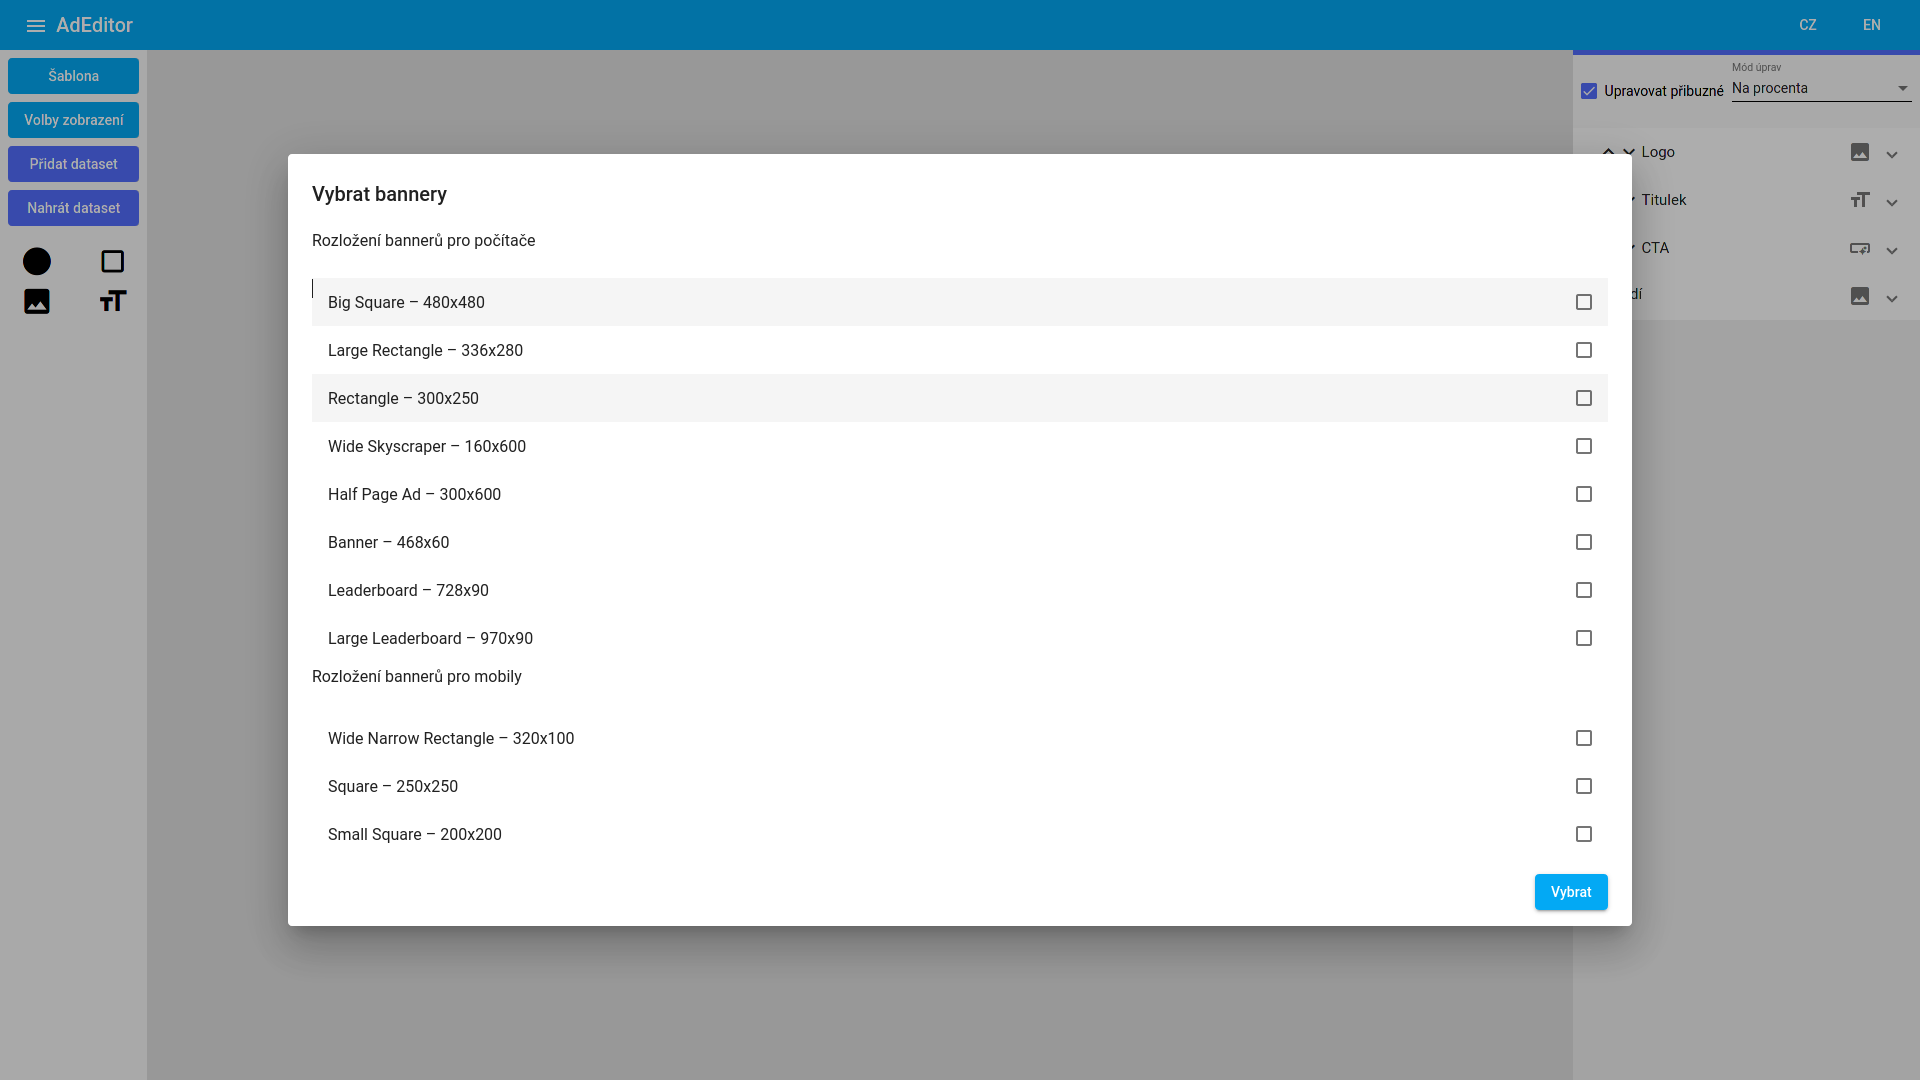
\includegraphics[width=1.0\textwidth]{Figures/editor/bannery-dialog.png}
        \caption[Výběr bannerů]{Dialogové okno pro výběr bannerů}
        \label{fig:editor:banner-dialog}
    \end{figure}

    \begin{figure}[h]
        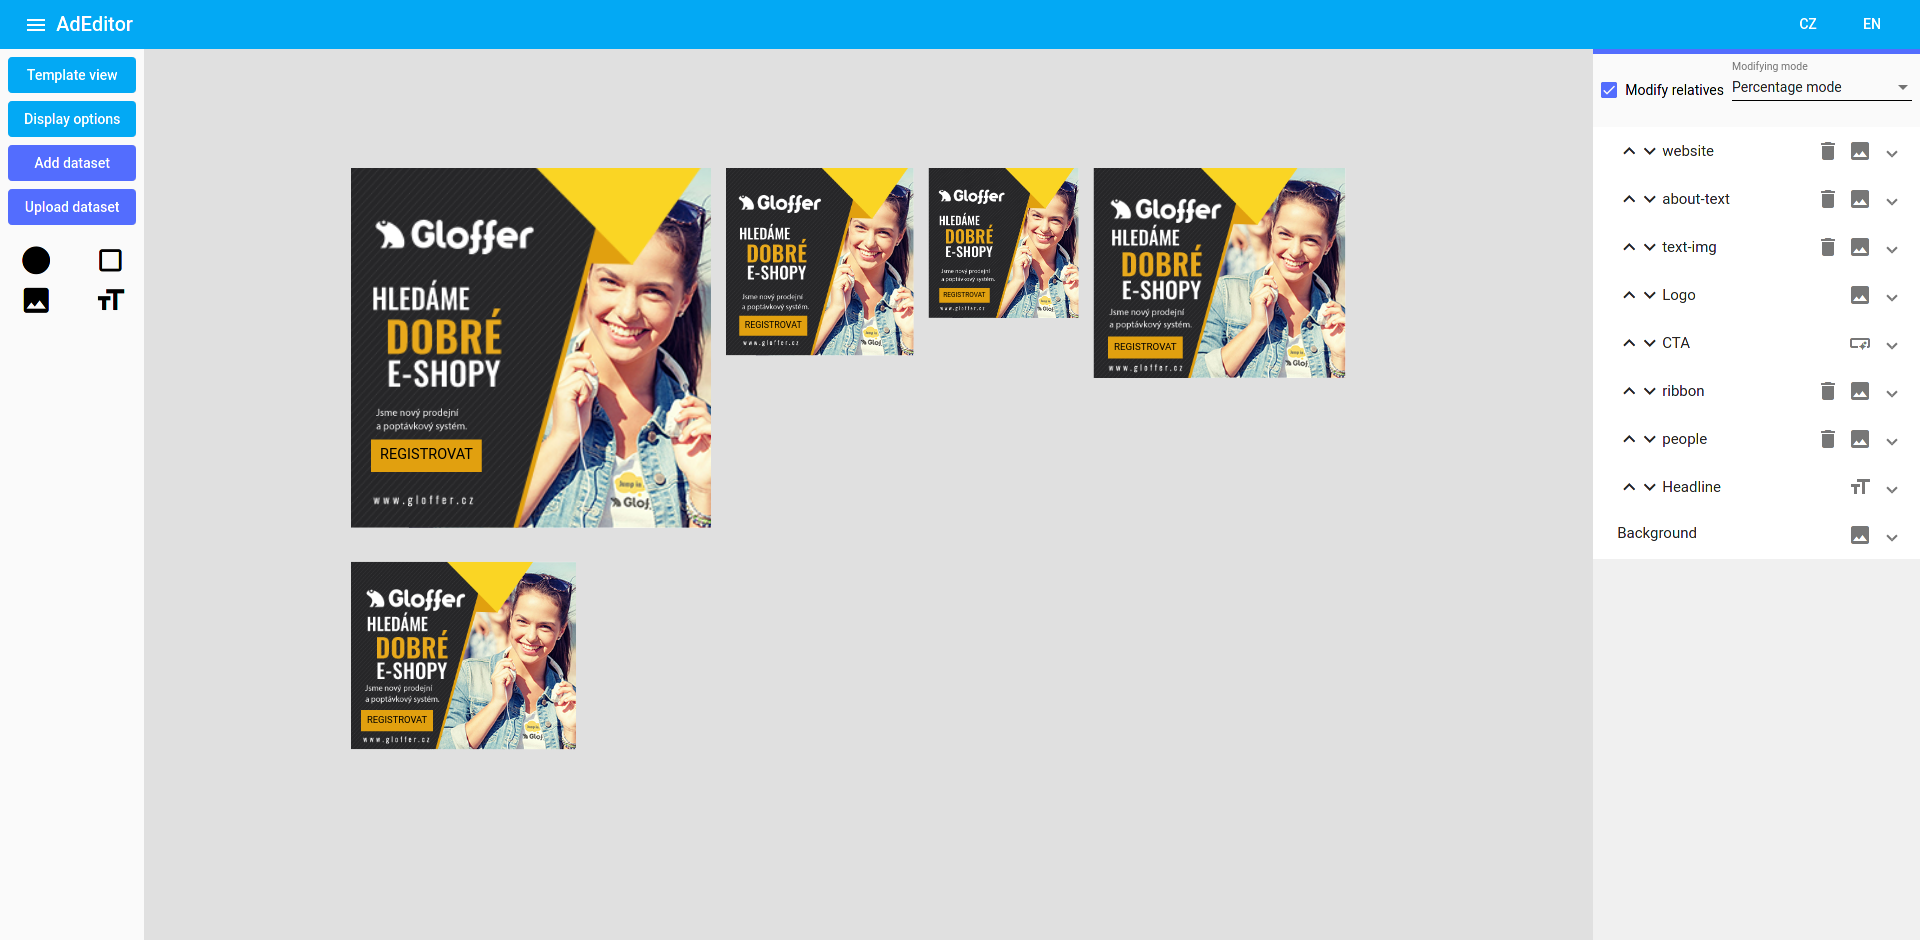
\includegraphics[width=1.0\textwidth]{Figures/editor/ad-editor-ui.png}
        \caption{Prostředí editoru}
        \label{fig:editor:editor}
    \end{figure}

    \begin{figure}[ht]
        \centering
        \begin{minipage}{.45\linewidth}
            \centering
            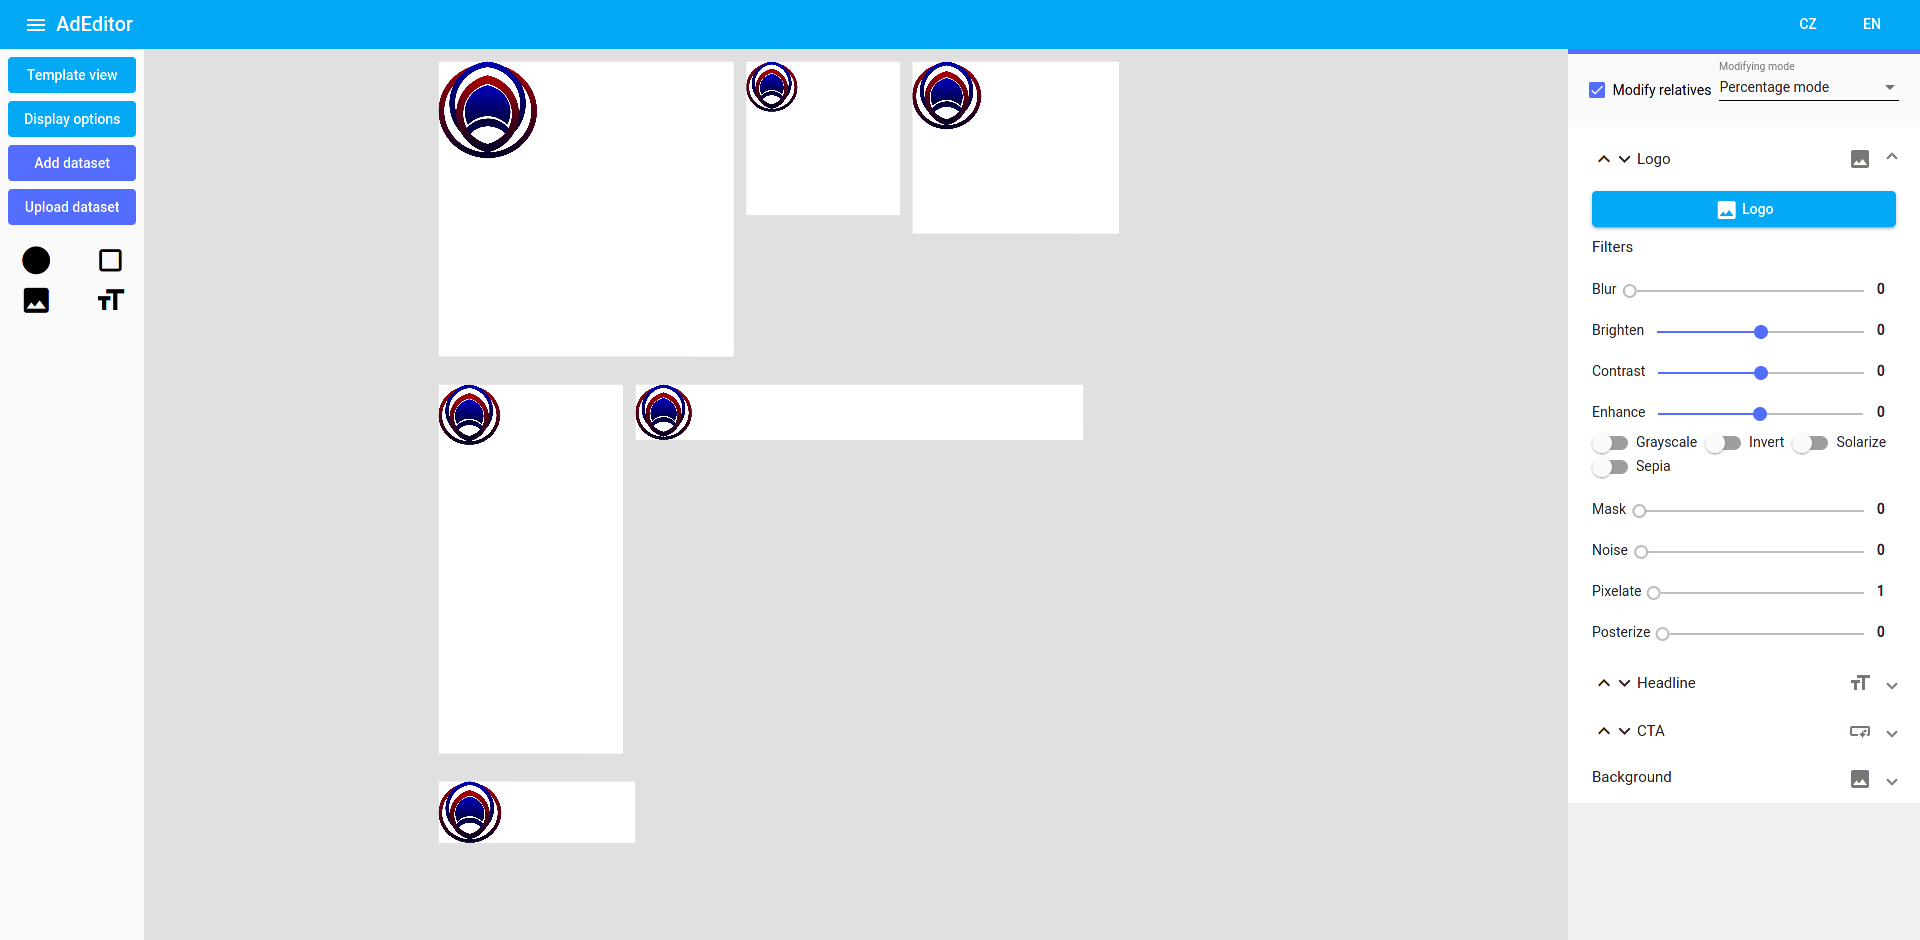
\includegraphics[width=1\textwidth]{Figures/editor/before-move.png}
            \caption{Stav před přetažením}
            \label{fig:editor:before-move}
        \end{minipage}
        \begin{minipage}{.45\linewidth}
            \centering
            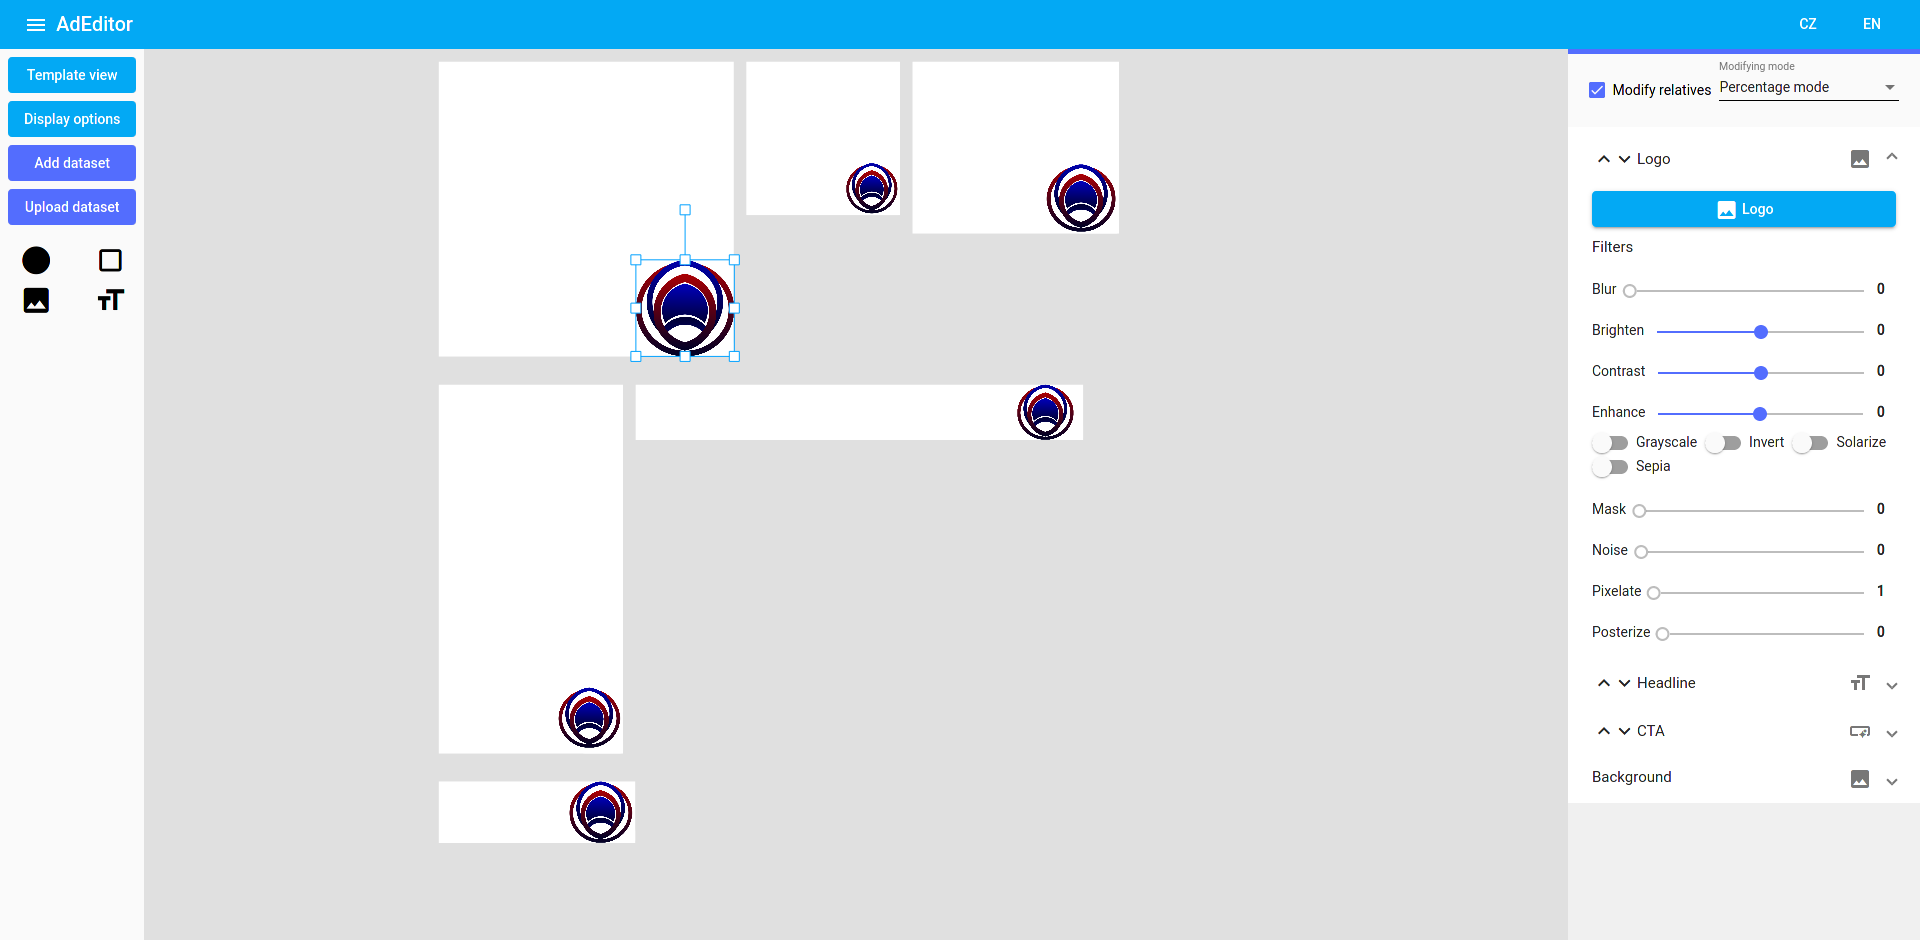
\includegraphics[width=1\textwidth]{Figures/editor/after-move.png}
            \caption{Stav po přetažení}
            \label{fig:editor:after-move}
        \end{minipage}
    \end{figure}

    \begin{figure}[h]
        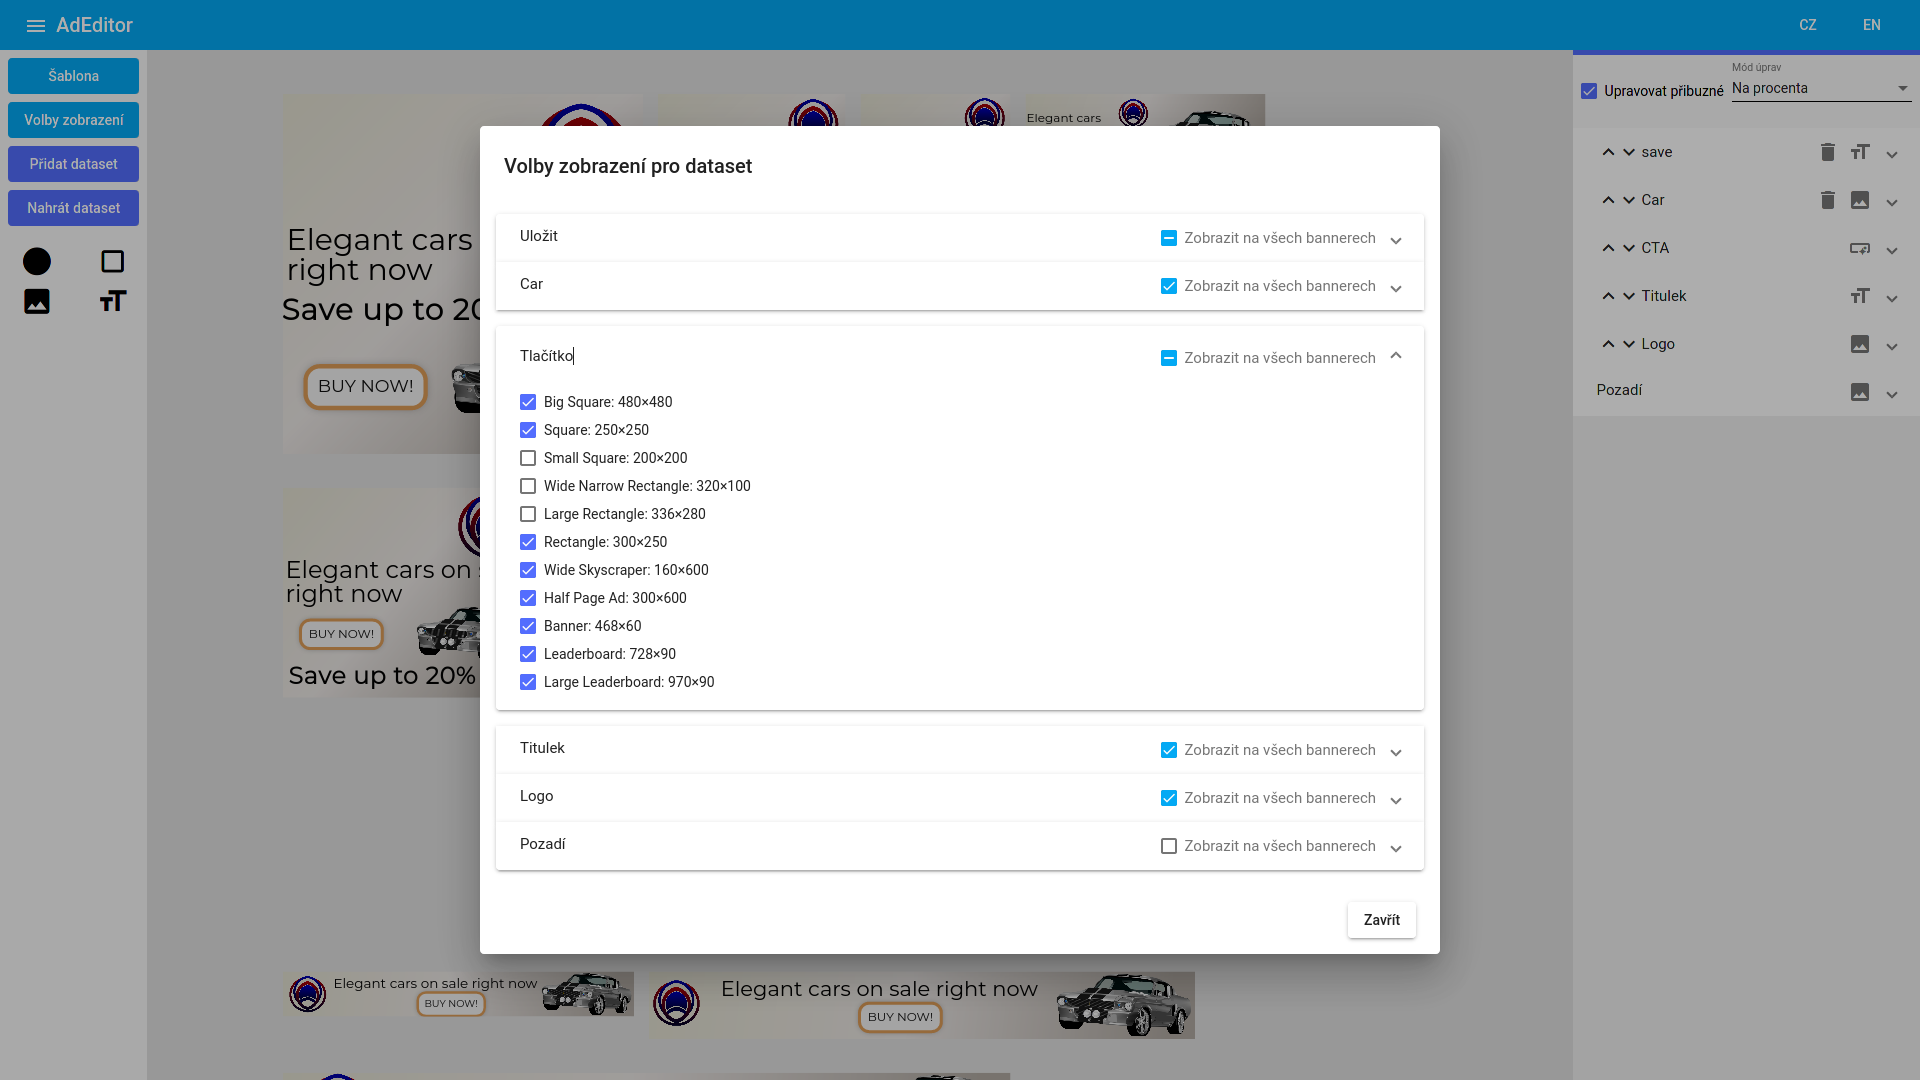
\includegraphics[width=1.0\textwidth]{Figures/editor/volby-zobrazeni.png}
        \caption[Volby zobrazení prvků]{Volby zobrazení na různých bannerech}
        \label{fig:editor:options}
    \end{figure}


    \begin{figure}[h]
        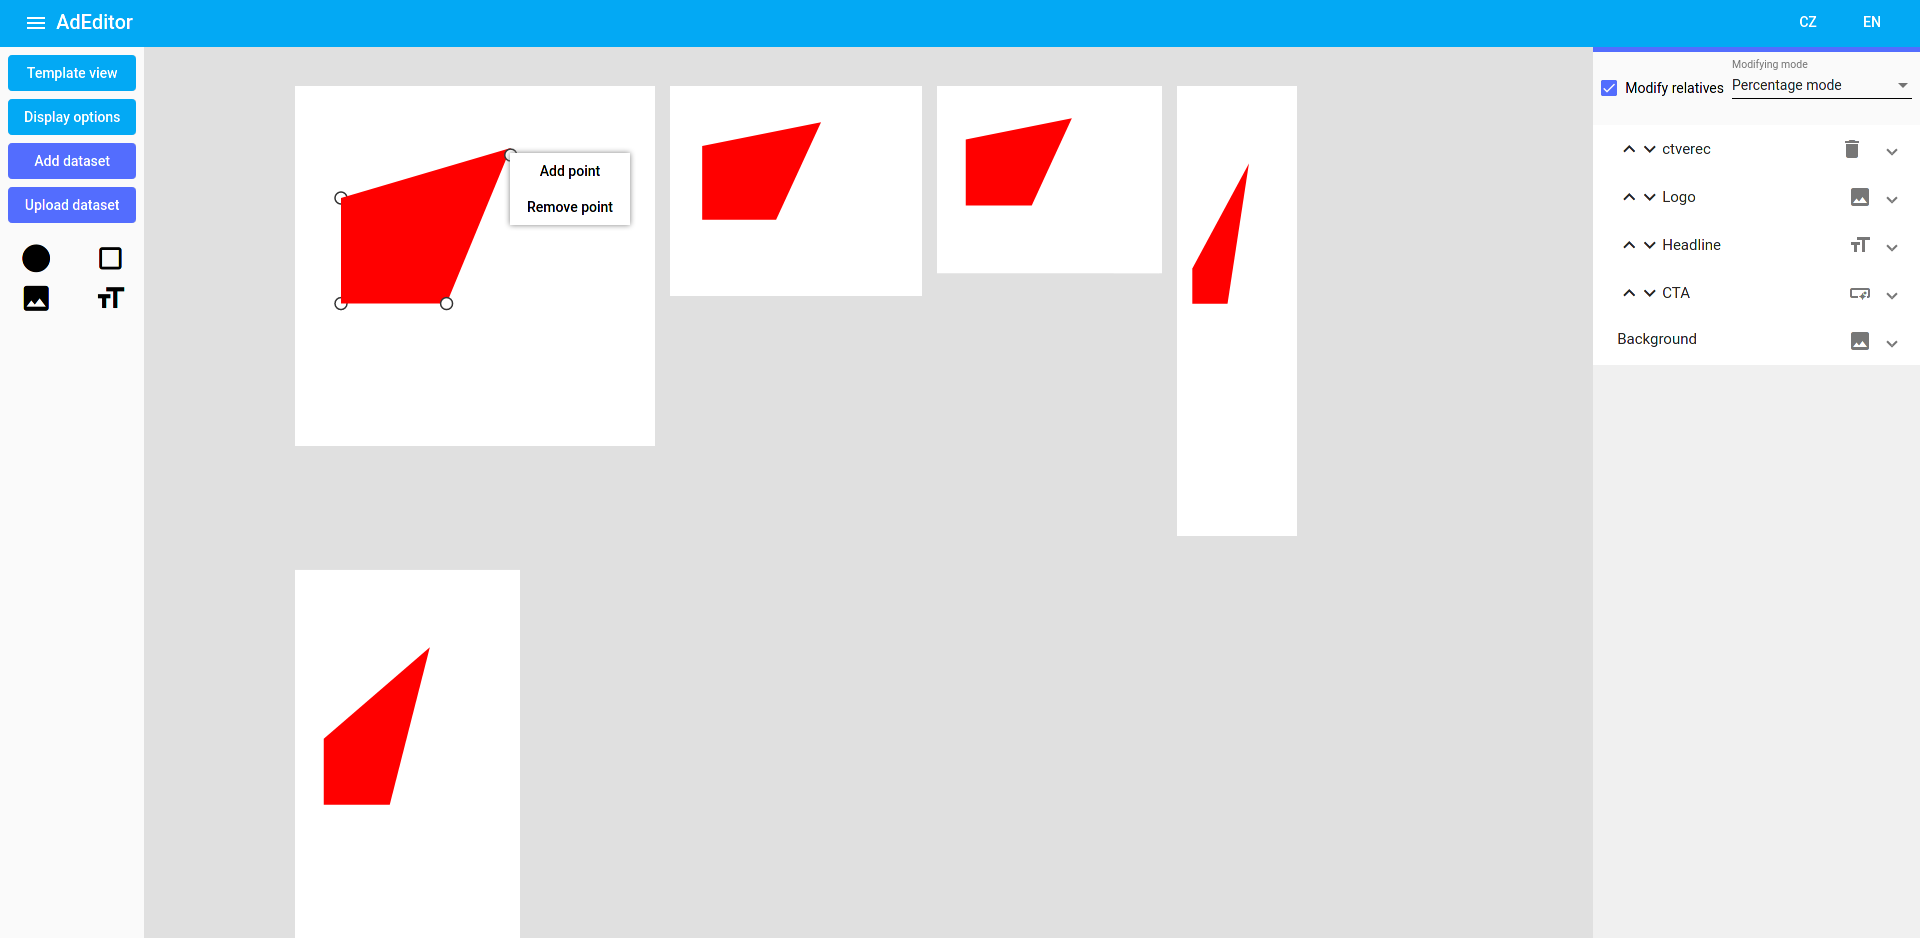
\includegraphics[width=1.0\textwidth]{Figures/editor/polygon.png}
        \caption{Úpravy mnohoúhelníku}
        \label{fig:editor:polygon}
    \end{figure}

\section{Nahrávání datasetů}
    Všechny vykreslované objekty musí být unikátně pojmenované.
    Poté je možno nahrát dataset ve formátu CSV. Jako hlavička CSV souboru musí být uvedeny názvy objektů, které si uživatel přeje změnit, v tzv.
    \emph{slugu}\footnote[2]{Slug je označení unikátního řetězce psaného malými písmeny a mezery nahrazené pomlčkou}. Měněné objekty mohou být pouze texty nebo zdroje obrázků. Obrázky aplikace umožňuje načítat i ze vzdálených zdrojů skrz 
    URL adresu, ale vzdálený server musí povolit \emph{CORS}. Po úspěšném nahrání se do aplikace tyto datasety přidají a lze mezi nimi přepínat. Každý
    dataset smí být individuálně dále upravován.

\section{Export bannerů}
    Jakmile je uživatel s výsledkem spokojen, umí bannery exportovat. Po zvolení exportu se zobrazí dialogové okno (obrázek \ref{fig:editor:exporting}) s nastavením exportu.
    Uživatel si může vybrat datasety k exportování, zda chce exportovat i šablonu, výstupní formát a případně poměr pixelů.
    Podporované výstupní formáty jsou JPEG a PNG. Pokud je zvolen JPEG, lze změnit i výslednou kvalitu.
    Dialog také zobrazuje největší odhadovanou velikost souboru, aby si uživatel nastavil vyhovující formát, případně kvalitu.
    Následně jsou vybrané datasety exportovány a staženy v ZIP archivu.

    \begin{figure}[h]
        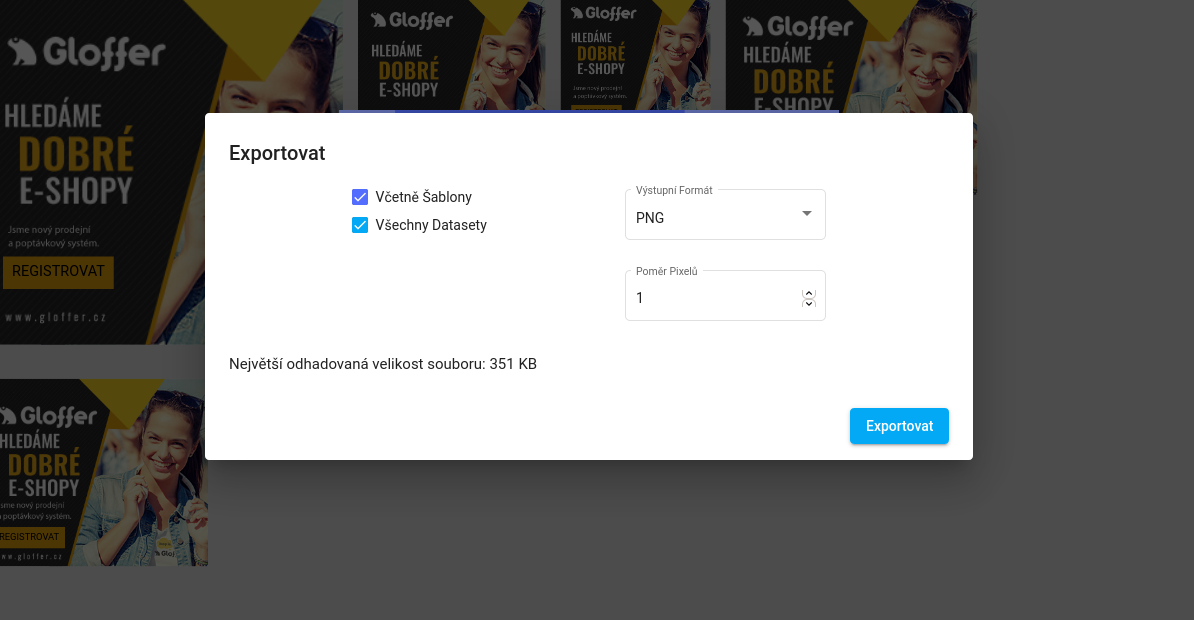
\includegraphics[width=1.0\textwidth]{Figures/editor/export.png}
        \caption{Dialogové okno pro export výsledných bannerů}
        \label{fig:editor:exporting}
    \end{figure}




\endinput